\documentclass[sigconf, anonymous]{acmart}

% is required for table formatting
\usepackage{array}

% for multi-line table cells
\usepackage{makecell}

\usepackage[ruled,vlined]{algorithm2e}

%% \BibTeX command to typeset BibTeX logo in the docs
\AtBeginDocument{%
  \providecommand\BibTeX{{%
    \normalfont B\kern-0.5em{\scshape i\kern-0.25em b}\kern-0.8em\TeX}}}

\begin{document}

\title{MeLES: Metric learning for event sequences with self-supervision}

\begin{abstract}

Constructing semantically meaningful embeddings from a huge amount of unlabelled lifestream data is a challenging representation learning problem. Those pre-trained embeddings incorporate complex information from the raw data as low-dimensional fixed-length vectors and could be easily applied in various downstream machine learning tasks as features. In this paper we propose a novel method to obtain lifestream data representation in the latent space based on metric learning approach. Traditionally, metric learning approach requires pairs of objects labeled as the same, but those pairs are often not available for lifestream data. So we propose a strategy based on subsequences generation from the raw data motivated by its periodicity and repeatability. 

We evaluated the proposed method over several public bank transactions datasets and showed that self-supervised embeddings are universal, can be applied to various downstream tasks and achieve performance results comparable to supervised methods. Moreover, embeddings are compact and exceptionally effective on datasets with limited label availability. 


\end{abstract}

\begin{CCSXML}
<ccs2012>
<concept>
<concept_id>10010147.10010257.10010293.10010294</concept_id>
<concept_desc>Computing methodologies~Neural networks</concept_desc>
<concept_significance>500</concept_significance>
</concept>
<concept>
<concept_id>10010405</concept_id>
<concept_desc>Applied computing</concept_desc>
<concept_significance>300</concept_significance>
</concept>
</ccs2012>
\end{CCSXML}

\ccsdesc[500]{Computing methodologies~Neural networks}
\ccsdesc[300]{Applied computing}

\keywords{representation learning, recurrent neural networks, temporal sequential data}

\maketitle

\section{Introduction}

In our research, we address the problem of leaning representations for event sequences generated by real-world users which we call \emph{lifestream} data. Event sequence data is produced in many business applications, some examples being credit card transactions and click-stream data of internet site visits, and the event sequence analysis is a very common machine learning problem~\cite{laxman2008stream},~\cite{wiese2009credit},~\cite{zhang2017credit},~\cite{bigon2019prediction}. Lifestream is an event sequence that is attributed to a person and captures his/her regular and routine actions of certain type, e.g., transactions, search queries, phone calls and messages.

In this paper, we present a novel method for the analysis of lifestreams that encodes event sequences of users by applying \emph{metric learning} techniques \cite{Hadsell:2006:DRL:1153171.1153654}.
Metric learning is often used for mapping high-dimensional objects to a low-dimensional embedding space. The aim of metric learning is to represent semantically similar objects, such as images, videos and audios, closer to each other, while dissimilar ones further. Most of the proposed metric learning methods have been applied to such fields as speech recognition \cite{wan2017generalized}, computer vision \cite{Schroff2015FaceNetAU}, \cite{Mao2019AdvRobust} and text analysis \cite{reimers-2019-sentence-bert}. 

In this paper we adopt metric learning to the analysis of event sequences by proposing a new \emph{Metric Learning for Event Sequences (MeLES)} method that encodes user lifestream data with low-dimensional embeddings and ... (**** EXPLAIN WHAT IT \textbf{DOES}. ALSO HOW DO YOU MEASURE MeLES'S PERFORMANCE? ****) 

The key property of the method is that it can be applied on unlabelled event sequences in a self-supervised manner.

{\bf Gleb's version of the above 2 paragraphs:}

{\bf AST: it reads more like an abstract or a one-page summary of the research (bez vodi :-)). USUALLY SUCH (KDD) PAPERS START WITH MOTIVATION OF THE PROBLEM AND ITS IMPORTANCE AND THEN GRADUALLY LEAD TO THE PROBLEM FORMULATION AND THE RESULTS.}

In this paper, we present a novel \emph{Metric Learning for Event Sequences (MeLES)} method for learning low-dimensional representations of event sequences, which copes with specific properties of lifestreams such as their discrete nature. In a broad sense, MeLES method adopts metric learning techniques~\cite{???}. Metric learning is often used in a supervised manner for mapping high-dimensional objects to a low-dimensional embedding space. The aim of metric learning is to represent semantically similar objects (images, video, audio, etc.) closer to each other, while dissimilar ones further. Most metric learning methods are used in such applications as speech recognition, computer vision, text analysis and reinforcement learning in 3D environments. In these domains, metric learning is successfully applied in a supervised manner to datasets, where pairs of high-dimensional instances are labeled as the same object or different ones. 
(*** AST: THE NEXT 2 SENTENCES CONSTITUTE A NICE AND CONCISE DESCRIPTION OF THE PROBLEM. THIS PIECE SHOULD BE KEPT AND INTEGRATED INTO THE PAPER. ***) Unlike all the previous metric learning methods, MeLES is fully self-supervised and does not require any labels. It is based on the observation that lifestream data obeys periodicity and repeatability of events in a sequence. Therefore, one can consider some convenient subsequences of the same lifestream as auxiliary high-dimensional representations of the same person. The idea of MeLES is that low-dimensional embeddings of such subsequences should be closer to each other.


Self-supervised learning have demonstrated effectiveness in different machine learning domains, such as Natural Language Processing (e. g. ELMO \cite{ELMO2018}, BERT \cite{Devlin2019BERTPO}) and computer vision \cite{doersch2015unsupervised}. The key advantage of self-supervised learning with respect to supervised learning is that it does not require labels, which can be expensive, limited or take time for collection. 
**** AST: THIS AND THE NEXT PARAGRAPH ARE CONFUSING AND SHOULD BE REWRITTEN. START WITH EXPLAINING WHAT "DOWNSTREAM TASKS" ARE AND HOW THEY ARE "REPRESENTED" IN THE MeLES MODEL. ***)
Self-supervised learning approach allows us to train rich models using the internal structure of large unlabelled or partially labeled training datasets. Knowledge, obtained through self-supervised learning, can be transferred to the downstream tasks via embedding extraction~\cite{word2vec} or fine-tuning~\cite{Devlin2019BERTPO}.

(*** AST: DO WE NEED TO EXPLAIN THIS IN THE INTRODUCTION? IS IT TOO SPECIFIC FOR THE INTRODUCTION? ***)
We initially trained the model in self-supervised way on public datasets with bank transactions and then evaluated MeLES either using the representation as features in the downstream task or fine-tuning the representation within a downstream task.

% MeLES can be used for compression of the event sequence to the fixed-size vector which is convenient for application in the downstream tasks.

MeLES representations achieve strong performance (*** AST: YOU HAVE NOT EXPLAINED WHAT THE MeLES PERFORMANCE IS    AND HOW YOU MEASURE IT ***) comparable to the baseline methods and  fine-tuned representations achieve state-of-the-art performance on both bank transactions datasets, outperforming several other supervised methods and methods with unsupervised pre-training by a significant margin.

Moreover, we show superiority of MeLES embeddings over supervised approach applied to partially labeled raw data due to insufficient amount of the target to learn a sufficiently complex model from scratch.

In this paper, we make the following contributions. We
\begin{enumerate}
    \item proposed to apply metric learning to the analysis of lifestream (event sequence) data in a self-supervised manner
    \item proposed a specific method, called Metric Learning for Event Sequences (MeLES), to accomplish this task 
    \item demonstrated that the proposed MeLES method significantly outperforms other baselines for both the supervised and the semi-supervised learning cases on lifestream data
\end{enumerate}

We provide the full source code for all experiments of the paper\footnote{https://github.com/***/*** (the link was anonymized for double-blind peer review)}.

\section{Related work} \label{sec-rel-work}

% We propose a method that uses metric learning approach as a self-supervised learning method for the lifestream domain. 
The metric learning approach used in our MeLES method has been widely used in different domains, including computer vision, NLP and audio domains. 

In particular, metric learning approach for imaging was proposed in \cite{Hadsell:2006:DRL:1153171.1153654}, where Contrastive loss function was used to learn a mapping of the input data to a low dimensional manifold with some prior knowledge of neighborhood relationships between training samples or manual labeling.

Furthermore, deep metric learning has been used for face recognition, \cite{Schroff2015FaceNetAU} introduced a FaceNet, which is learning a mapping from face images to a Euclidean compact 128-D embedding using a triplet- based loss function based on LMNN \cite{weinberger2006distance} and proposing online triplet selection and training procedure based on hard-positive and hard-negative mining technique. 

Recently, metric learning was applied to increase the robustness of images representation for adversarial attacks \cite{Mao2019AdvRobust}, where triplet loss function was used to pull the images of similar class, both natural and adversarial, closer while pushing the images of other classes far apart. 

Also, metric learning has been used for the speaker verification task \cite{wan2017generalized}, where the contrast loss is defined as embedding of each utterance being similar to the centroid of all that speaker's embeddings (positive pair) and far from other speaker's centroids with the highest similarity among all false speakers (hard negative pair).

In \cite{reimers-2019-sentence-bert} was proposed a fine-tuned BERT model \cite{Devlin2019BERTPO} that use siamese and triplet network architectures to train sentence embeddings using semantic proximity annotation of sentence pairs.

Although metric learning was used in all these domains, it has not been applied to the analysis of the lifestream problems involving transactional, click-stream and other types of lifestream data, which is the focus of this paper.

As explained in Section 1???, the MeLES method applies metric learning to the event sequence domain using self-supervised learning. 
The idea of applying self-supervised learning to sequential data has been previously proposed in Contrastive Predictive Coding (CPC) method \cite{DBLP:journals/corr/abs-1807-03748}, where
meaningful representations are extracted by predicting future in the latent space by using autoregressive methods. CPC representations demonstrated strong performance on four distinct domains: audio, computer vision, natural language and reinforcement learning.

In computer vision domain there are many other different approaches to self-supervised learning that are nicely summarized in \cite{jing2019selfsupervised}.

Note that almost every self-supervised learning approach can be reused for the representation learning in the form of embeddings. There are several examples of using a single set of embeddings for several downstream tasks \cite{Song2017LearningUE}, \cite{Zhai:2019:LUE:3292500.3330739}.
Embeddings have long history of successful usage in NLP applications to represent documents as a fixed-length vectors. There are some efforts to generalize embeddings approaches for more broad cases \cite{Wu2017StarSpaceEA}.
A common approach to learn self-supervised representations is either traditional autoencoder (\cite{rumelhart1985learning}) or variational autoencoder (\cite{kingma2013auto}). It is widely used for images, text and audio or aggregated lifestream data (\cite{mancisidor2019learning}).

Although self-supervised learning has been successfully used in several domains listed above, it has not been applied to the raw lifestream data in the form of event sequences, mainly due to the challenges of defining distances between the input and the reconstructed input data.

In the next section we describe how metric learning is applied to the event sequences in a self-supervised manner.

\section{Method} \label{sec-method}

\subsection{Lifestream data}

We designed the method specially for the lifestream data. Lifestream data consists of discrete events per user (or other entities) in continuous time, for example, user behavior on websites, credit card transactions, etc. 

Considering credit card transactions, each transaction have a set of attributes, either categorical or numerical including the timestamp of the transaction. An example of the sequence of three transactions with their attributes is presented in the Table \ref{tab-tr-data}.
Merchant type field represents the category of a merchant, such as "airline", "hotel", "restaurant", etc.

\begin{table}[ht]
\caption{Data structure for a single credit card}
\begin{tabular}{ | m{7em} |  m{5em} m{5em} m{5em}| }
\hline
\textbf{Amount} & 230 & 5 & 40 \\
\textbf{Currency} & EUR & USD & USD \\
\textbf{Country} & France & US & US \\
\textbf{Time} & 16:40 & 20:15 & 09:30 \\
\textbf{Date} & Jun 21 & Jun 21 & Jun 22 \\
\textbf{Merchant Type} & Restaurant & Transport\-ation & Household Appliance \\
\hline
\end{tabular}
\label{tab-tr-data}
\end{table}

Another example of lifestream data is click-stream: the log of internet pages  visits. The example of a click-stream log of a single user is presented in Table \ref{tab-cs-data}.

\begin{table}[ht]
\caption{Click-stream structure for a single user}
\begin{tabular}{ | m{2em} m{3em} m{7em} m{10em} | }
\hline
\textbf{Time} & \textbf{Date} & \textbf{Domain} & \textbf{Referrer Domain} \\
\hline
17:40 & Jun 21 & amazon.com & google.com \\
17:41 & Jun 21 & amazon.com & amazon.com \\
17:45 & Jun 21 & en.wikipedia.org & google.com \\
\hline
\end{tabular}
\label{tab-cs-data}
\end{table}

\subsection{General framework}

\begin{figure*}[ht]
  \caption{General framework}
  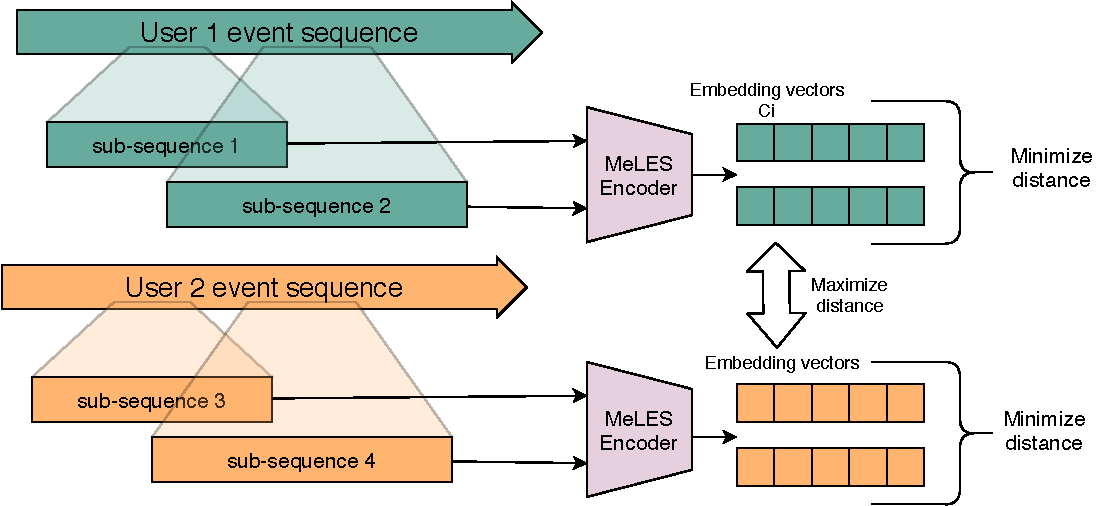
\includegraphics[scale=0.9]{figures/arch-v2.pdf}
  \label{fig-arch}
\end{figure*}

The overview of the method is presented at figure \ref{fig-arch}. Given a sequence of discrete events $\{x_t \}^T_{t=1}$ in a given observation interval [1, T] the ultimate goal is to obtain a sequence embedding $c_t$ for the timestamp $T$ in the latent space $R^d$. To train the encoder to generate meaningful embedding $c_t$ from $\{x_t \}^T_{t=1}$ we apply a metric learning approach such that the distance between embeddings of the similar user or entity (positive pairs) is small, whereas embeddings of the different users or entities (negative pairs) is large.

One of the difficulties with applying metric learning approach to the lifestream data is that the notion of semantic similarity as well as dissimilarity requires underlying domain knowledge and human labor-intensive labeling process to constrain positive and negative examples. 
The key property of the lifestream data domain is periodicity and repeatability of the events in the sequence which allows us to reformulate the metric learning task in a self-supervised manner. MeLES learns low-dimensional embeddings from user' sequential data, sampling positive pairs as sub-sequences of the same user' sequence and negative pairs as sub-sequences from different user' sequences. See section \ref{sec-pos-pairs}) for the details of the positive pairs generation.

Embedding $c_t$ is generated by encoder neural network which is described in section \ref{sec-enc-arch}. The details of the metric learning loss are described in section \ref{sec-ml-loss}. The details of the positive pairs generation strategies are described in section \ref{sec-pos-pairs}. The details of the negative pairs sampling strategy is described in section \ref{sec-neg-samples}.

Sequence embedding $c_t$ obtained by the metric learning approach is then used in various donwstream machine learning tasks as a feature vector. Also, it is possible to improve the downstream task performance is to feed a pre-trained embedding $c_t$ (e. g. the last layer of RNN) to a task-specific classification subnetwork and then jointly fine-tune the model parameters of the encoder and classifier subnetworks.

\subsection{Encoder architecture} \label{sec-enc-arch}

To embed a sequence of events as the fixed-size vector $c_t \in R^d$ we use the approach similar to the E.T.-RNN card transaction encoder proposed in \cite{10.1145/3292500.3330693}. The whole encoder network consists of two conceptual parts: the event encoder and the sequence encoder subnetworks.

The event encoder $e$ takes the set of attributes of a single event and outputs its representation in the latent space $Z \in R^m$: $z_t = e(x_t)$. The sequence encoder $s$ takes latent representations of the sequence of events: $ z_{1:T} = z_1, z_2, \cdots z_T $ and outputs the representation of the whole sequence $c_t$ in the time-step t: $ c_t = s(z_{1:t}) $.

The event encoder consists of the several embedding layers and batch normalization\cite{10.5555/3045118.3045167} layer. Each embedding layer is used to encode each categorical attribute of the event. Batch normalization is applied to numerical attributes of the event. Finally, outputs of every embedding layer and batch normalization layer are concatenated to produce the latent representation $z_t$ of the single event.

The sequence of latent representations of event representations $z_{1:t}$ is passed to sequence encoder $s$ to obtain a fixed-size vector $c_t$. Several approaches can be used to encode a sequence. One possible approach is to use the recurrent network (RNN) as in \cite{Sutskever:2014:SSL:2969033.2969173}. The other approach is to use the encoder part of the Transformer architecture presented in \cite{DBLP:journals/corr/VaswaniSPUJGKP17}. In both cases the output produced for the last event can be used to represent the whole sequence of events. In case of RNN the last output $h_t$ is a representation of the sequence.

Encoder, based on RNN-type architecture like GRU\cite{cho2014learning}, allows to calculate embedding $c_{t+k}$ by updating embedding $c_t$ instead of  calculating embedding $c_{t+k}$ from the whole sequence of past events $z_{1:t}$: $c_k = rnn(c_t, z_{t+1:k})$. This option allows to reduce inference time when you need to update already existing client embeddings with new events, occurred after the calculation of embeddings. This is possible due to the recurrent nature of RNN-like networks.

\subsection{Metric learning losses} \label{sec-ml-loss}

Metric learning loss discriminates embeddings such that embeddings from similar class are moved closer together and embeddings from the different class are moved further. Several metric learning losses have been considered - Contrastive Loss \cite{Hadsell:2006:DRL:1153171.1153654}, Binomial Deviance Loss \cite{Yi:2014:LUE:1407.4979}, Triplet Loss \cite{Hoffer:2015:LUE:1412.6622}, Histogram Loss \cite{histogram-loss} and Margin Loss \cite{wu2017sampling}. All of this losses address the following challenge of the metric learning approach: using all pairs of samples is inefficient, for example, some of the negative pairs are already distant enough thus this pairs are not valuable for the training (\cite{simo2015discriminative}, \cite{wu2017sampling}, \cite{Schroff2015FaceNetAU}).

In the next paragraphs we will consider two kinds of losses, which are conceptually simple, and yet demonstrated strong performance on validation set in our experiments (see Table \ref{tab-loss-type}), namely Contrastive Loss and Margin loss.

Contrastive loss has a contrastive term for the negative pair of embeddings which penalizes the model only if the negative pair is not distant enough and the distance between embeddings is less than the margin $m$:  
\begin{equation}
 \mathcal{L} = \sum_{i=1}^P \left[ (1-Y)\dfrac{1}{2}(D_W^i)^2 +Y*\dfrac{1}{2}\{max(0,m-D_W^i)\}^2 \right],
\end{equation}
where $P$ is the count of all pairs in a batch, $D_W^i$ - is a distance function between a i-th labeled sample pair of embeddings $\vec{X_1}$ and $\vec{X_2}$, 
$Y$ is a binary label assigned to a pair: $Y = 0$ means a similar pair, $Y = 1$ means dissimilar pair, $m > 0$ is a margin.
As proposed in \cite{Hadsell:2006:DRL:1153171.1153654} we use euclidean distance as the distance function: $D_W^i(\vec{A},\vec{B}) = \sqrt{\sum_i(\vec{A_i} - \vec{B_i})^2}$.

Margin loss is similar to the Contrastive loss, the main difference is that there is no penalty for positive pairs which are closer than threshold.
\begin{equation}
 \mathcal{L} = \sum_{i=1}^P \left[ (1-Y)max(0, D_W^i - b + m) + Y*max(0, b-D_W^i + m) \right],
\end{equation}
where $P$ is the count of all pairs in a batch, $D_W^i$ - is a distance function between a i-th labeled sample pair of embeddings $\vec{X_1}$ and $\vec{X_2}$,
$Y$ is a binary label assigned to a pair: $Y = 0$ means a similar pair, $Y = 1$ means dissimilar pair, $m > 0$ and $b > 0$ define the bounds of a margin.

\subsection{Negative sampling} \label{sec-neg-samples}

Negative sampling is another way to address the issue that some of the negative pairs are already distant enough thus this pairs are not valuable for the training (\cite{simo2015discriminative}, \cite{wu2017sampling}, \cite{Schroff2015FaceNetAU}). Hence, only part of possible negative pairs are considered during loss calculation. Note, that only current batch samples are considered. There are several possible strategies of selecting most relevant negative pairs.

\begin{enumerate}
    \item Random sample of negative pairs
    \item Hard negative mining: generate k hardest negative pairs for each positive pair.
    \item Distance weighted sampling, where negative samples are drawn uniformly according to their relative distance from the anchor. \cite{wu2017sampling}
    \item Semi-hard sampling, where we choose the nearest to anchor negative example, from samples which further away from the anchor than the positive exemplar (\cite{Schroff2015FaceNetAU}).
\end{enumerate}

In order to select negative samples, we need to compute pair-wise distance between all possible pairs of embedding vectors of a batch. In order to make this procedure more computationally effective we perform normalisation of the embedding vectors, i. e. project them on a hyper-sphere of unit radius. Since $D_W^i(\vec{X},\vec{Y}) = \sqrt{\sum_i(\vec{X_i} - \vec{Y_i})^2} = \sqrt{\sum_i\vec{X_i}^2 + \sum_i\vec{Y_i}^2 - 2\sum_i\vec{X_i}\vec{Y_i}} $ and $||\vec{X}||= ||\vec{Y}||=1$, to compute the the euclidean distance we only need to compute: $D_W^i = \sqrt{2 - 2\sum_i\vec{X_i}\vec{Y_i}}$.

To compute the dot product between all pairs in a batch we just need to multiply the matrix of all embedding vectors of a batch by itself, which is a highly optimized computational procedure in most modern deep learning frameworks. Hence, the computational complexity of the negative pair selection is $O(n^2h)$ where $h$ is the size of the output embeddings and $n$ is the size of the batch.

\subsection{Positive pairs generation} \label{sec-pos-pairs}

The following procedure is used to create a batch during MeLES training. $N$ initial sequences are taken for batch generation. Then, $K$ sub-sequences are produced for each initial sequence.

Pairs of sub-sequences produced from the same sequence are considered as positive samples and pairs from different sequences are considered as negative samples. Hence, after positive pair generation each batch contains $N \times K$ sub-sequences used as training samples, there are $K-1$ positive pairs and $(N - 1) \times K$ negative pairs per sample in batch.

There are several possible strategies of sub-sequence generation. The simplest strategy is the random sampling without replacement. Another strategy is to produce a sub-sequence from random splitting sequence to several sub-sequences without intersection between them (see Algorithm \ref{alg-disj-ss}). The third option is to use randomly selected slices of events with possible intersection between slices (see Algorithm \ref{alg-slce-ss}).

\begin{algorithm}
\SetAlgoLined
\textbf{hyperparameters:} $k$ - amount of sub-sequences to be produced. \\
\textbf{input:} A sequence $S$ of length $l$. \\
\textbf{output:} $S_1,...,S_k$ - sub-sequences from $S$. \\

\BlankLine
Generate vector $inds$ of length $l$ with random integers from [1,k].\\
 \For{$i\leftarrow 1$ \KwTo $k$}{
 $S_i = S[inds == i]$
 }
 \caption{Disjointed sub-sequences generation strategy}
\label{alg-disj-ss}

\end{algorithm}

\begin{algorithm}
\SetAlgoLined
\textbf{hyperparameters:} $m, M$ - minimal and maximal possible length of sub-sequence. $k$ - amount of sub-sequences to be produced. \\
\textbf{input:} A sequence $S$ of length $l$. \\
\textbf{output:} $S_1,...,S_k$ - sub-sequences from $S$. \\
\BlankLine
 \For{$i\leftarrow 1$ \KwTo $k$}{
 Generate random integer $l_i$, $m \leqslant l_i \leqslant \min(M,l).$\\
 Generate random integer $s$, $0 \leqslant s \leqslant l-l_i.$\\
 $S_i = S[s: s + l_i]$
 }
 \caption{Random slices sub-sample generation strategy}
\label{alg-slce-ss}
\end{algorithm}

Note, that the order of events in generated sub-sequences is always preserved.

\section{Experiments} \label{sec-exp}

\subsection{Datasets} \label{sec-datasets}
In our research we used several publicly available datasets of bank transactions.
\begin{enumerate}
    \item \textbf{Age group prediction competition}\footnote{https://onti.ai-academy.ru/competition} - the task is to predict the age group of a client within 4 classes target and accuracy is used as a performance metric.
    The dataset consists of 44M anonymized transactions representing 50k clients with a target labeled for only 30k of them (27M out of 44M transactions), for the other 20k clients (17M out of 44M transactions) label is unknown. Each transaction includes date, type (for example, grocery store, clothes, gas station, children's goods, etc.) and amount. We use all available 44M transactions for metric learning, excluding 10\% - for the test part of the dataset, and  5\% for the metric learning validation.
        
    \item \textbf{Gender prediction competition}\footnote{https://www.kaggle.com/c/python-and-analyze-data-final-project/} - the task is a binary classification problem of predicting the gender of a client and ROC-AUC metric is used.
    The dataset consists of 6,8M anonymized transactions representing 15k clients, where only 8,4k of them are labeled. Each transaction is characterized by date, type (for ex. "ATM cash deposit"), amount and Merchant Category Code (also known as MCC).
\end{enumerate}

\subsection{Experiment setup}

For each dataset, we set apart 10\% clients from the labeled part of data as the test set that we used for comparing different models.

If we do not explicitly mention alternative, in our experiments we use contrastive loss and random slices pair generation strategy.

For all methods hyper-parameters were chosen using random search on 5-fold cross-validation over the train set in point of best out-of-fold performance on train set.

The final set of hyper-parameters used for MeLES is shown in the Table\ref{tab-hyper}.

\begin{table}[ht]
\caption{Hyper-parameters for MeLES training}
\begin{tabular}{ | m{18em} |  m{3em} | m{3em} | }
\hline
& \textbf{Age task} & \textbf{Gender task} \\
\hline
\textbf{Learning rate} & 0.002 & 0.002 \\
\textbf{Number of samples in batch} & 64 & 128 \\
\textbf{Number of epochs} & 100 & 150 \\
\textbf{Number of generated sub-samples} (see Section \ref{sec-pos-pairs}) & 5 & 5 \\
\hline
\end{tabular}
\label{tab-hyper}
\end{table}

For evaluation of semi-supervised/self-supervised techniques (including MeLES), we used all transactions including unlabeled data, but except for the test set, as far this methods are suitable for partially labeled datasets, or don't require labels at all.

\subsubsection{Performance}

Neural network training was performed on a single Tesla P-100 GPU card. For the training part of MeLES the single training batch is processed in 142 millisecond. For age prediction dataset the single training batch contains 64 unique clients with 5 subsamples per client, i. e. 320 training samples in total, the mean number of transactions per sample is 90, hence each batch contains around 28800 transactions.

\subsubsection{Baselines} \label{sec-baselines}

In order to compare our method with baselines, we decided to concider two methdos Gradient Boosting Machine (GBM) method \cite{friedman2001} on hand-crarted features and Contrastive Predictive Coding (CPC) \cite{cp}. Hence, we decided to adapt successful approaches from other tasks, namely Gradient Boosting Machine (GBM) method \cite{friedman2001} on hand-crarted features. prediction and CPC.

To compare metric learning based model with other approaches, we have implemented an
additional model that is based on the Gradient Boosting Machine
(GBM) method \cite{friedman2001} and Contrastive predictive coding.
GBM based model require a large number of hand-crafted aggregate features produced from the transactional data as an input to the classification model. An example
of an aggregate feature would be an average spending amount in
some category of merchants, such as hotels of the entire transaction
history.
We used LightGBM\cite{NIPS2017_6907} implementation of GBM algorithm with nearly 1k hand-crafted features for the application.

We use following approach to feature creation. Features are created on client level based on his all transactions. We split attributes of each transaction to categorical (like 'mcc code', 'trx type', ...) and numeric (amount). First group of features based on numeric attributes. We calculate some aggregates over all values for each attributes. As aggregate functions we use 'sum', 'mean', 'std', 'min', 'max'. As we have only one numeric field (amount), we have 5 features in first group. Second group of features based on combination of categorical and numeric attributes. We group numeric values by categorical values. Aggregate functions is 'count', 'mean', 'std'. As for age prediction task we have one categorical attribute (small group) with 200 unique values, combining it with amount we can produce $200 * 3$ features ('group0 x amount x count',  'group1 x amount x count', ..., 'group199 x amount x count', 'group0 x amount x mean', ...). In total we use approx 605 features for age prediction task. For gender prediction task we have two categorical features: 'mcc code' with approx 200 unique values and 'tr type' with approx 100 unique values. So in total we use $200 * 3 + 100 * 3 + 5 = 905$ features.

Such features contains detailed information about client spending profile but omit temporal information.

We also compare MeLES with another embedding generation method: Contrastive predictive coding.

Although self-supervised learning has been successfully used in several domains listed above, it has not been applied to the raw lifestream data in the form of event sequences, mainly due to the challenges of defining distances between the input and the reconstructed input data.

\subsubsection{Design choices}

In the Table\ref{tab-enc-type}, Table\ref{tab-loss-type}, Table\ref{tab-pair-gen} and Table\ref{tab-neg-sampl} we present the results of experiments on different design choices of our method.

As shown in Table\ref{tab-enc-type}, different choices of encoder architectures show comparable performance on the downstream tasks.

It is interesting to observe that even Contrastive loss that can be considered as the basic variant of metric learning loss allows to get strong results on the downstream tasks (see Table \ref{tab-loss-type}). Our hypothesis is that increase in the model performance on metric learning task is not always lead to increase in performance on downstream tasks.

Also observe that hard negative mining leads to significant increase in quality on downstream tasks in comparison to random negative sampling (see Table\ref{tab-neg-sampl}).

Another observation is that more complex sub-sequence generation strategy shows same performance as random sampling of events on the considered downstream tasks (see Table\ref{tab-pair-gen}).

\begin{table}[ht]
\caption{Comparison of encoder types}
\begin{tabular}{ | m{10em} |  m{7em} | m{7em} | }
\hline
\textbf{Econder type} & \makecell{\textbf{Age,} \\ \textbf{Accuracy $\pm 95\%$}} & \makecell{\textbf{Gender,} \\ \textbf{AUROC $\pm 95\%$}} \\
\hline
\textbf{LSTM} & $0.620 \pm 0.003$ & $0.870 \pm 0.005$ \\
\textbf{GRU} & \pmb{$0.639 \pm 0.006$} & \pmb{$0.871 \pm 0.004$}  \\
\textbf{Transformer} & $0.621 \pm 0.001$ & $0.848 \pm 0.002$  \\
\hline
\end{tabular}
\label{tab-enc-type}
\end{table}

\begin{table}[ht]
\caption{Comparison of metric learning losses}
\begin{tabular}{ | m{10em} |  m{7em} | m{7em} |}
\hline
\textbf{Loss type} & \makecell{\textbf{Age,} \\ \textbf{Accuracy $\pm 95\%$}} & \makecell{\textbf{Gender,} \\ \textbf{AUROC $\pm 95\%$}} \\
\hline
\textbf{Contrastive loss} & $0.639 \pm 0.006$ & \pmb{$0.871 \pm 0.003$} \\
\textbf{Binomial Deviance loss} & $0.535 \pm 0.005$ & $0.853 \pm 0.005$ \\
\textbf{Histogram loss} & \pmb{$0.642 \pm 0.002$} & $0.851 \pm 0.004$ \\
\textbf{Margin loss} & $0.631 \pm 0.003$ & \pmb{$0.871 \pm 0.004$} \\
\textbf{Triplet loss} & $0.610 \pm 0.006$ & $0.855 \pm 0.003$ \\
\hline
\end{tabular}
\label{tab-loss-type}
\end{table}

\begin{table}[ht]
\caption{Comparison of pair generation strategies}
\begin{tabular}{ | m{10em} |  m{7em} |  m{7em} | }
\hline
\textbf{Pair generation method} & \makecell{\textbf{Age,} \\ \textbf{Accuracy $\pm 95\%$}} & \makecell{\textbf{Gender,} \\ \textbf{AUROC $\pm 95\%$}} \\
\hline
\textbf{Random samples} & $0.628 \pm 0.003$ & $0.851 \pm 0.004$ \\
\textbf{Random disjoint samples} & $0.608 \pm 0.004$ & $0.836 \pm 0.008$ \\
\textbf{Random slices} & \pmb{$0.639 \pm 0.006$} & \pmb{$0.872 \pm 0.005$}  \\
\hline
\end{tabular}
\label{tab-pair-gen}
\end{table}

\begin{table}[ht]
\caption{Comparison of negative sampling strategies}
\begin{tabular}{ | m{10em} |  m{7em} |  m{7em} | }
\hline
\textbf{Negative sampling strategy} & \makecell{\textbf{Age,} \\ \textbf{Accuracy $\pm 95\%$}} & \makecell{\textbf{Gender,} \\ \textbf{AUROC $\pm 95\%$}} \\
\hline
\textbf{Hard negative mining} & \pmb{$0.637 \pm 0.005$} & \pmb{$0.872 \pm 0.004$} \\
\textbf{Random negative sampling} & $0.615 \pm 0.005$ & $0.826 \pm 0.004$ \\
\textbf{Distance weighted sampling} & $0.620 \pm 0.003$ & $0.867 \pm 0.003$ \\
\hline
\end{tabular}
\label{tab-neg-sampl}
\end{table}

\begin{figure}[ht]
  \caption{Embedding dimensionality vs. quality for age prediction task}
  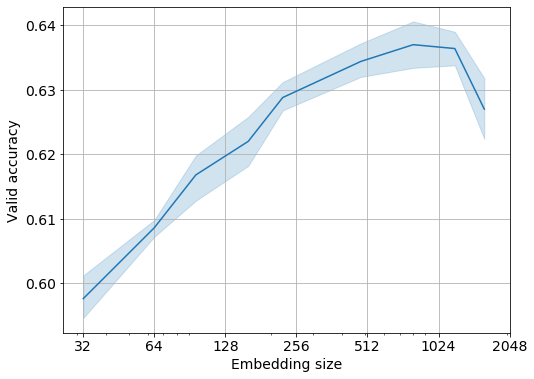
\includegraphics[width=0.46\textwidth]{figures/age-pred-hidden-size.png}
  \label{fig-emb-dim-age}
\end{figure}

\begin{figure}[ht]
  \caption{Embedding dimensionality vs. quality for gender prediciton task}
  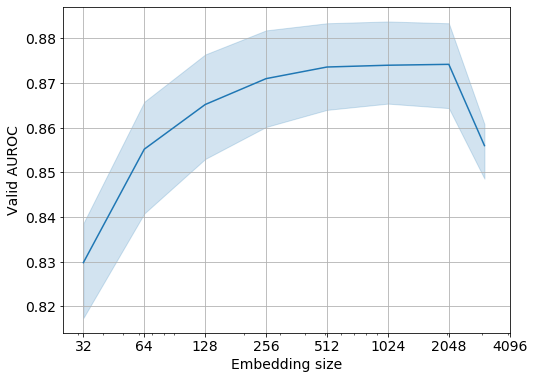
\includegraphics[width=0.46\textwidth]{figures/gender-hidden-size.png}
  \label{fig-emb-dim-gender}
\end{figure}

We tried to estimate embedding dimensionality which leads to better quality on downstream task. We found that bigger embedding store more information about original sequence and leads to better quality on downstream task. But making embeddings longer we reach cuda out of memory error. We can decrease batch size to fit long vectors into memory.

At Figure \ref{fig-emb-dim-age} we can see that accuracy on downstream task grows with bigger embeddings. The best quality is achieved at size 800. Further increase in embedding reduces quality.
It seems to be standard bias-variance trade-off. When dimensionality is too small, it seems that too much signal power is discarded (high bias). On the
other hand, when dimensionality is too large, too much noise is included (high variance).

At Figure \ref{fig-emb-dim-gender} we see the similar dependency. We can found a plateau between 256 and 2048, when quality don't increase. We choose embedidng size = 256.

Note, that increasing embedding size we also increase a training time.


\subsubsection{Embedding visualization}

We calculate embedding via MeLES model. We receive 800-dimensional vectors for age prediction dataset and 256-dimensional vectors for gender prediction dataset. Next we apply tSNE transformation and convert vectors to 2-d coordinates. tSNE transforms high-dimensional space to low-dimensional based on local relationships between points. So neighbour vectors in embedding space are pushed to be close in 2-d space.

Now we can colorize points based on target values. Note, that embeddings was obtained without target information. The MeLES model builds vectors only from raw client transactions. Sequence of transaction can be mentioned like client behavior. The MeLES model capture information about behavioral patterns and put the similar patterns nearby. As shown below, this local areas in embedding space may be correspond to some clients attributes like age or gender.

tSNE points for age prediction task shown on Figure \ref{fig-tsne-age}. We can see a good enough division of vectors into 4 groups. Bins '1' and '2' are on opposite side of cloud. Bins '2' and '3' are in the middle. Taking care that age is ordinal attribute, we can suppose such relations between bins: $age(1) < age(3) < age(0) < age(2)$ (or reversal), where $age(bin)$ returns age of client for specific bin.

tSNE points for gender prediction task shown on Figure \ref{fig-tsne-gender}. There are areas dominated by one gender label over another.

This results shows generalizing ability of MeLES model.

\begin{figure}[ht]
  \caption{2D tSNE mapping of MeLES embeddings trained on age prediction task dataset, colored by age group labels}
  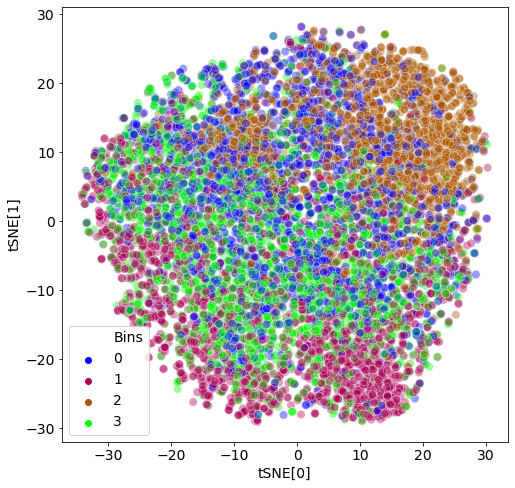
\includegraphics[width=0.46\textwidth]{figures/age-pred-tsne.png}
  \label{fig-tsne-age}
\end{figure}

\begin{figure}[ht]
  \caption{2D tSNE mapping of MeLES embeddings trained on gender prediction task dataset, colored by gender labels}
  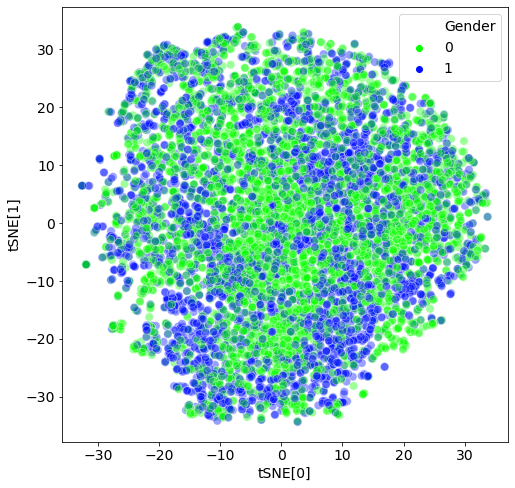
\includegraphics[width=0.46\textwidth]{figures/gender-tsne.png}
  \label{fig-tsne-gender}
\end{figure}

\subsection{Results} \label{sec-res}

\subsubsection{Comparison with baselines} \label{sec-res-baselines}

As shown in Table \ref{tab-age-pred} and Table \ref{tab-sex-pred} our method generates sequence embeddings of lifestream data that achieve strong performance, comparable to performance on manually crafted features when used on downstream tasks. Also fine-tuned representations obtained by our method achieve state-of-the-art performance on both bank transactions datasets, outperforming all previous learning methods by a significant margin.

Also note, that the usage of sequence embedding together with hand-crafted aggregate features leads to better performance than usage of only hand-crafted features or sequence embeddings, i. e. it is possible to combine different approaches to get even better model.


\begin{table}[ht]
\caption{Age group prediction results}
\begin{tabular}{ | m{18em} |  m{6em} | }
\hline
\textbf{Method} & \textbf{Accuracy $\pm 95\%$} \\
\hline
\textbf{LightGBM on hand-crafted features} & $0.626 \pm 0.004$ \\
\textbf{LightGBM on Metric Learning embeddings} & $0.639 \pm 0.006$ \\
\textbf{LightGBM on both hand-crafted features and Metric Learning embeddings} & $0.643 \pm 0.009$ \\
\textbf{Supervised learning} & $0.631 \pm 0.010$  \\
\textbf{MeLES fine-tuning} & \pmb{$0.643 \pm 0.007$}  \\
\textbf{LightGBM on CPC embeddings} & $0.595 \pm 0.004$  \\
\textbf{Fine-tuned Contrastive Predictive Coding} & $0.621 \pm 0.007$  \\
\hline
\end{tabular}
\label{tab-age-pred}
\end{table}

\begin{table}[ht]
\caption{Gender prediction results}
\begin{tabular}{ | m{18em} |  m{6em} | }
\hline
\textbf{Method} & \textbf{AUROC $\pm 95\%$} \\
\hline
\textbf{LightGBM on hand-crafted features} & $0.875 \pm 0.004$ \\
\textbf{LightGBM on Metric Learning embeddings} & $0.872 \pm 0.005$ \\
\textbf{LightGBM on both hand-crafted features and Metric Learning embeddings} & $0.882 \pm 0.003$ \\
\textbf{Supervised learning} & $0.871 \pm 0.007$  \\
\textbf{MeLES fine-tuning} & \pmb{$0.888 \pm 0.002$} \\
\textbf{LightGBM on CPC embeddings} & $0.848 \pm 0.004$  \\
\textbf{Fine-tuned Contrastive Predictive Coding} & $0.873 \pm 0.007$  \\
\hline
\end{tabular}
\label{tab-sex-pred}
\end{table}

\subsubsection{Semi-supervised setup} \label{sec-semi}

To evaluate our method in condition of a restricted amount of labeled data we use only part of available target labels for the semi-supervised experiment.
As well as in supervised setup we compare proposed method with ligthGBM over hand-crafted features and Contrastive Predictive Coding (see Section \ref{sec-baselines}).
For both embedding generation methods (our MeLES and CPC) we evaluate performance of the lightGBM on embeddings and performance of fine-tuned on downstream task models on part of the data.
In addition to this baselines we compare our method with supervised learning on available part of the data.

In figures \ref{fig-semi-age-0} and \ref{fig-semi-gender-0} we compare the quality of various features by learning lightGBM on top of them. Moreover, in figures \ref{fig-semi-age-1} and \ref{fig-semi-gender-1} one can find comparison of a single models trained on both downstream tasks considered in this paper. As you can see, in conditions of limited labeled data, our method are superior to the other approaches.

\begin{figure}[ht]
  \caption{Age group prediction task quality on features for different dataset sizes}
  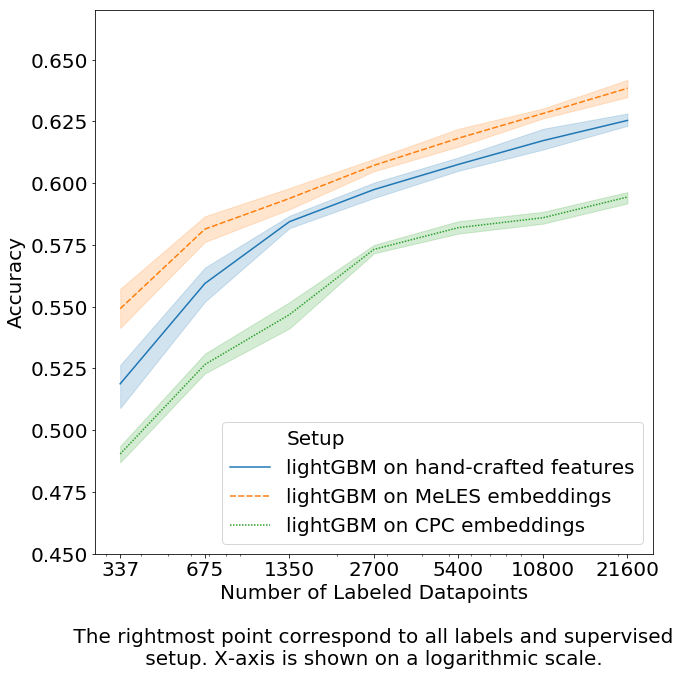
\includegraphics[width=0.46\textwidth]{figures/ss_age_0.png}
  \label{fig-semi-age-0}
\end{figure}

\begin{figure}[ht]
  \caption{Gender prediction task quality on features for different dataset sizes}
  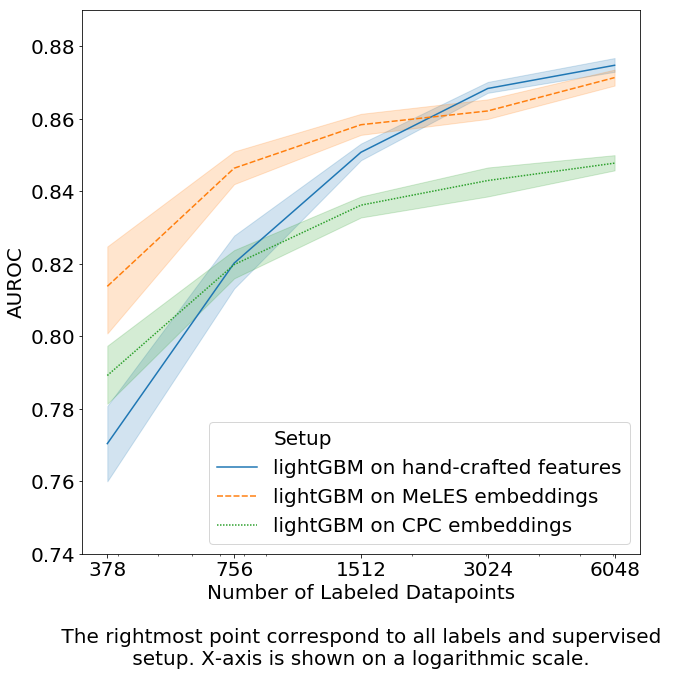
\includegraphics[width=0.46\textwidth]{figures/ss_gen_0.png}
  \label{fig-semi-gender-0}
\end{figure}

\begin{figure}[ht]
  \caption{Age group prediction task quality of single model for different dataset sizes}
  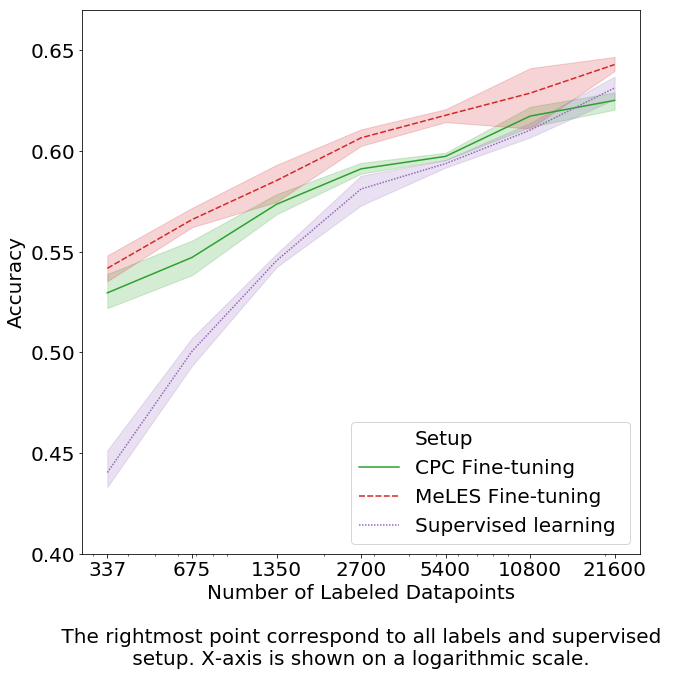
\includegraphics[width=0.46\textwidth]{figures/ss_age_1_wopl.png}
  \label{fig-semi-age-1}
\end{figure}

\begin{figure}[ht]
  \caption{Gender prediction task quality of single model for different dataset sizes}
  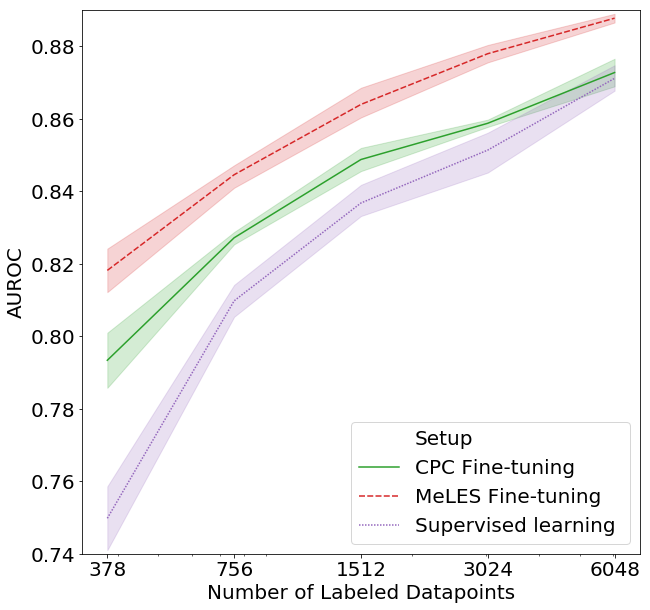
\includegraphics[width=0.46\textwidth]{figures/ss_gen_1.png}
  \label{fig-semi-gender-1}
\end{figure}

\section{Conclusions} \label{sec-conclusions}

In this paper we propose to apply metric learning to the analysis of the lifestream data in a self-supervised manner. As a part of this proposal, we developed the Event sequence metric learning (MeLES) method that is based on self-supervised learning. 
In particular, the MeLES method can be used to produce embeddings of complex event sequiences that can be effectively used in various downstream tasks. Also, our method can be used for pre-training in semi-supervised settings.

We also empirically demonstrate that our approach achieves strong performance results on several downstream tasks by significantly (???) outperforming both classical machine learning baselines on hand-crafted features and neural network based approaches.
In the semi-supervised setting, where the number of labelled data is limited, our method demonstrates even stronger results: it outperforms other methods by significant margins.

The proposed method of generating embeddings is convenient for production usage since almost no pre-processing is needed for complex event streams in order to get compact embeddings of that streams. The pre-calculated embeddings can then be easily used for different downstream tasks without performing complex and time-consuming computations on the raw event data. For some encoder architectures, such as those presented in Section \ref{sec-enc-arch}, it is even possible to incrementally update the already calculated embeddings when additional new lifestream data arrives. Overall, the usage of universal precalcuated embeddings allows to democratize the usage of large amounts of data along analysts (AST: ???) in an organization.

Another advantage of using sequence-based (AST: event-based???) embeddings, instead of the raw explicit event data, is that it is impossible to restore the exact input sequence from its embeddings. Therefore, the usage of embeddings leads to better privacy and data security for the end users than when working directly with the raw event data, and all this is achieved without sacrificing valuable modelling power.
**** AST: DID YOU PUT THIS LAST STATEMENT IN THE INTRODUCTION WHEN LISTING THE ADVANTAGES OF THE MeLES METHOD? ****


\bibliographystyle{ACM-Reference-Format}
\bibliography{sigconf}

\end{document}
